\chapter{Gait Watch and Qualisys Optica motion tracker}
\label{ch:GWandQS}

\section{Introduction and chapter's structure}
After explaining and comparing both Gait Watch and Force Plate systems, we proceed now to do an analysis of the differences and similarities between Gait Watch and the Qualisys Optical motion tracker.

It has been demonstrated that Qualisys System is an accurate system to analyse the body movements and it can be used in several applications. However, this system has a lot of constraints like the possibility of application scope.

Thus, we are going to do a comparison with the Gait Watch system, a system based on inertial sensors being more portable and cheaper.
Along this chapter we will explain how the pitch angle has been calculated using the Qualisys System. That is, we will compare with the angles obtained through inertial sensors.


\section{Computing Euler angles using Qualisys System}
To compute the Euler angle, the subject is wearing two infrared markers per segment placed on both thighs and shanks. The infrared optical cameras emit infrared light and this reflects in the markers placed over the body allowing to know the position of the markers.

The pitch angle of such segment is computed between the vector defined by the upper and lower markers and the vector normal to the Earth’s surface. To be able to compute it we first have to define a third point which has the same X coordinate as the lower marker and the same Z coordinate as the upper marker. This will define a right triangle in which one of the contiguous cathetus is normal to the Earth’s surface and the hypotenuse is defined by the line between the upper and the lower point. Therefore, by calculating the arctangent we can easily find the angle of the right triangle, which is, in turn, the pitch angle\cite{OlivaresBotzel2013}. We can see this in \ref{fig:pitchQS}

\begin{figure}[H]
	\centering
	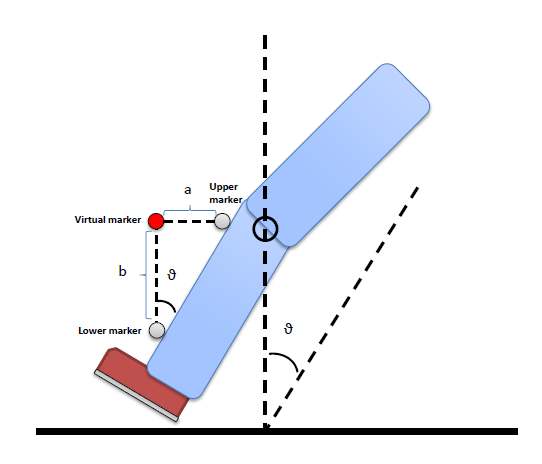
\epsfig{file=imagenes/pitchQS, width=1\textwidth}
	\caption{Diagram of the pitch computation using the Qualisys System \cite{OlivaresBotzel2013}.}
	\label{fig:pitchQS}
\end{figure}

Thus, the pitch angle is computed as follows:

\begin{equation}
\label{angleQS1}
	\theta_{QS}= arctang(\frac{a}{b})
\end{equation}

\begin{equation}
\label{angleQS2}
	a= \sqrt{(x_{upper}-x_{lower})^{2} + (z_{upper}-z_{upper})^{2} }
\end{equation}

\begin{equation}
\label{angleQS3}
	b= \sqrt{(x_{lower}-x_{lower})^{2} + (z_{lower}-z_{upper})^{2} }
\end{equation}

where $ [x_{lower}, z_{lower} ] $ and $ [x_{upper}, z_{upper} ] $ are the coordinates of the projections of the lower an upper markers in the XZ plane, respectively.

\section{Feature extraction}
In this experiment, prior to start the data gathering, we set up the protocol that people have to carry out while the data are recorded. Seven control subjects have been involved. They had to walk during some minutes over a treadmill with different speeds, specifically 2, 4 and 6 Km/h.

This movement is characterised by the Gait Watch system and the Qualisys System. To do this, the participants wear the inertial sensors over the body and the infrared markers, being these last ones visible by infrared cameras all the time. This experiment is carried out in a control environment where both systems can work properly.

Once the data have been gathered, we process them before the applying the feature extraction. For the GW signals, the procedure is the same than in aforementioned cases. The first step is doing the calibration and correct the erroneous values in the signals due to a noise of the sensors.
Then, we can figure out the angle of the different segments of the body. The program done in Matlab allows us to choose what segments we can use to calculate and compare between both systems. In this case, we can select: right shank, left shank, right thigh and left thigh.

The angle of these segments are calculated for each point of time with a sample frequency of 200 samples/s for both systems so we don’t have to interpolate because these signals match perfectly. The pitch is filtered with a Kalman Filter in the GW signals because it is an algorithm that uses measurements observed over the time and produces estimates of unknown variables that tend to be more precise than others base on a single measurement. In other words, Kalman Filter operates recursively on stream of noisy inputs data to produce a statistically optimal state of the underlying system state\cite{Kalman Filter}.

Hereafter, we calculate the pitch using the QS signals. To to this, we will apply the equations described in the prior chapter \ref{angleQS1}.
After this, we have to center all of these signals and we will be ready to compare all signals now.

\begin{figure}[H]
	\centering
	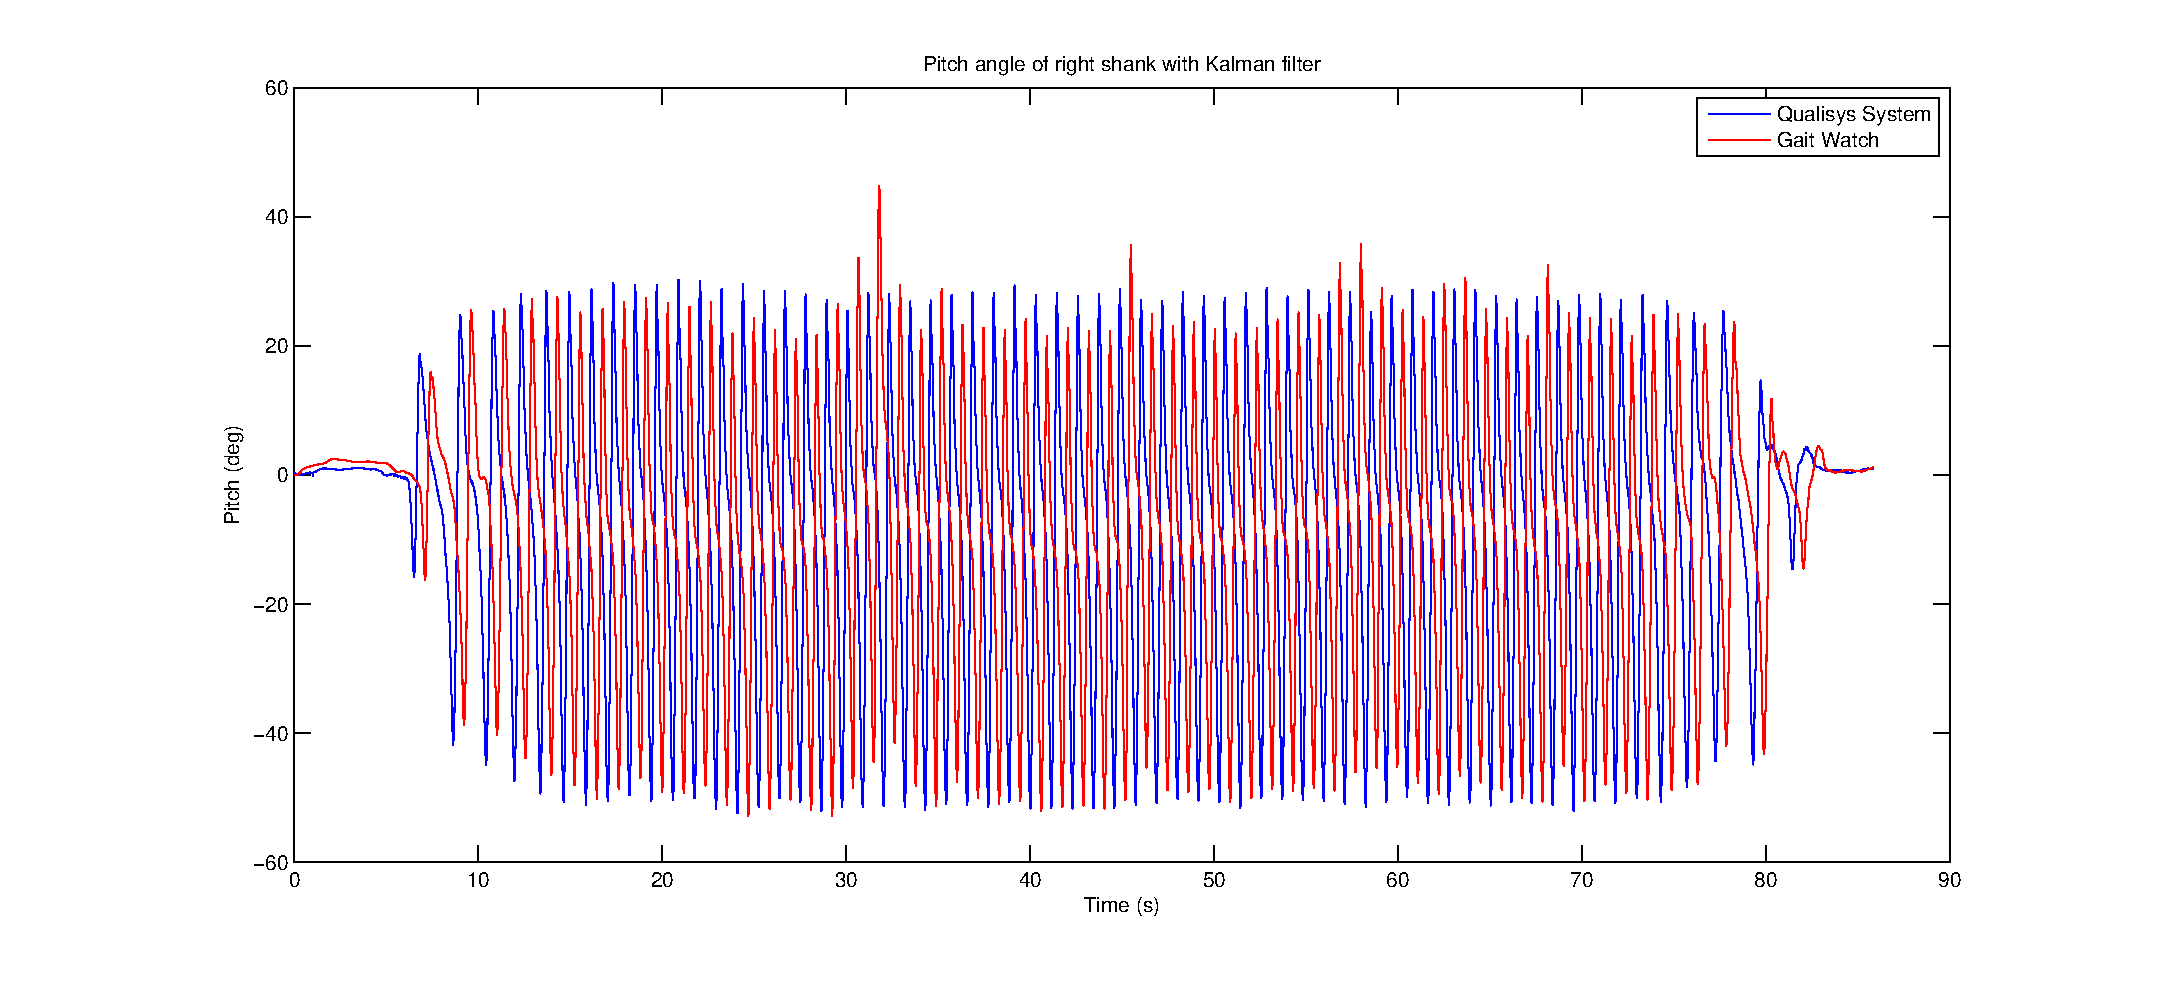
\epsfig{file=figures/QSvsGW/signalGWQS, width=1\textwidth}
	\caption{Pitch angle of right shank for 4Km/h of speed.}
	\label{fig:signalGWQS}
\end{figure}

The next step is the feature extraction. We have to differentiate two comparison. Firstly, we are going to compare the pitch calculated with inertial sensors (GW) and infrared cameras (QS), so we will extract some specific characteristics to do this. After, we are going to compare the angle obtained in function of the speed.
\begin{figure}[H]
	\centering
	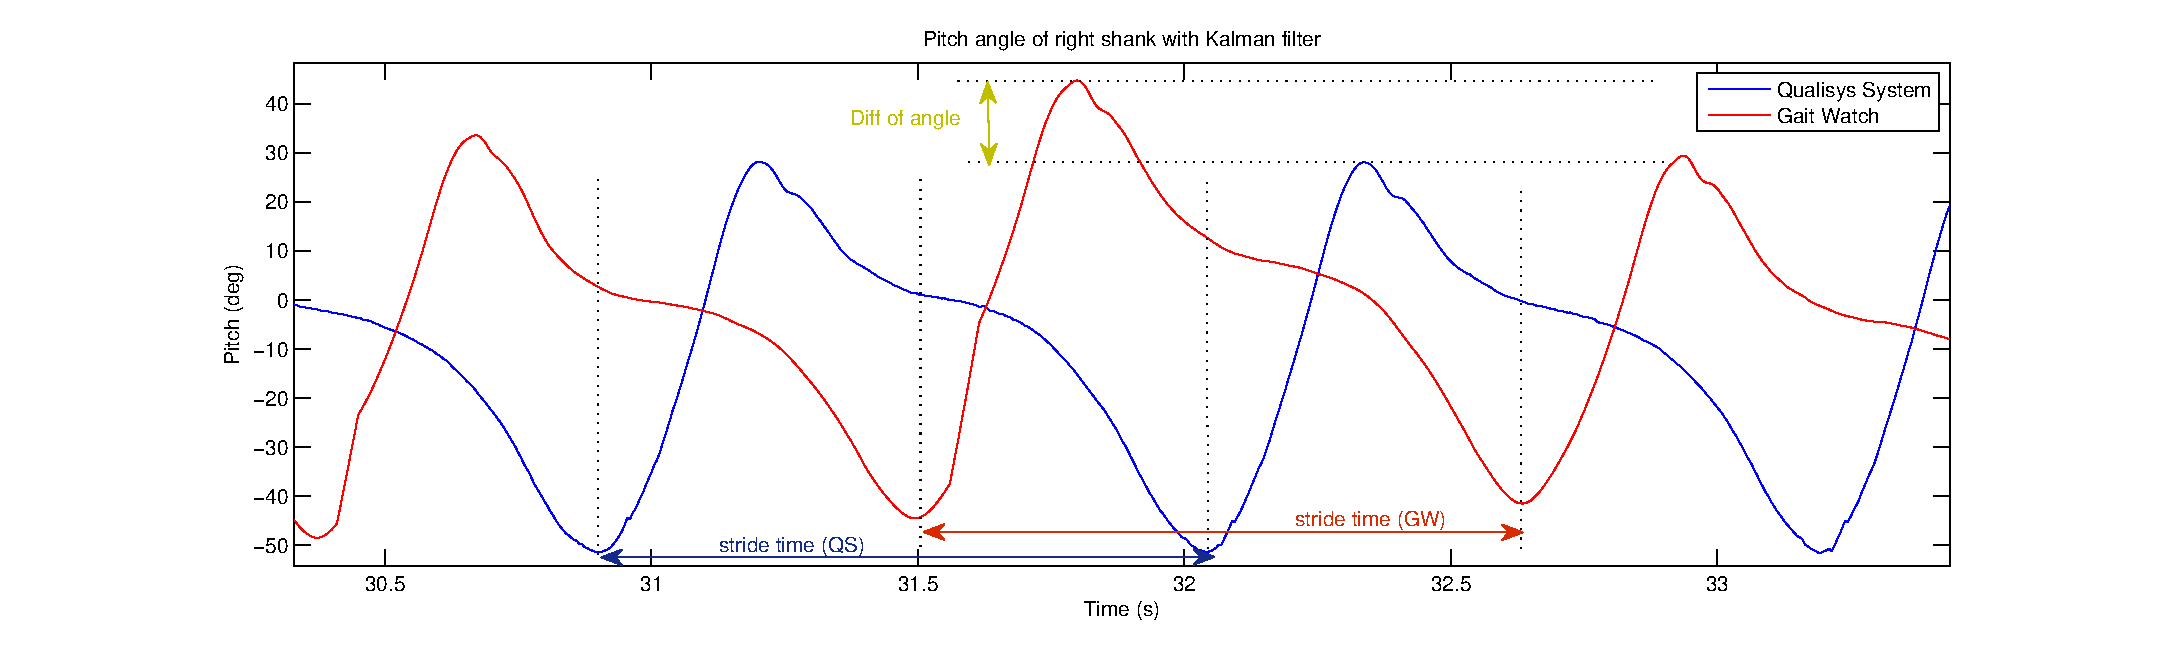
\epsfig{file=figures/QSvsGW/features_GWQS, width=1\textwidth}
	\caption{Features for pitch angle in GW and QS signals.}
	\label{fig:featuresGWQS}
\end{figure}
The first feature computed was the ‘stride time’ \ref{fig:featuresGWQS}. This is the time that a person needs to carry out a step, i.e the time since the foot is lifted from the treadmill until the moment when the same foot touches the ground and gains momentum to step again. In the pitch signal, we determine this detecting the distance between two negative value of the pitch because the negative values happen when the segment (shank or thigh) are behind the trunk, this is just before stepping.

Other important aspect is the difference of angle obtained in both systems. We calculate values positives as well as negatives and finally obtain the mean of the difference of all them \ref{fig:featuresGWQS}.


\section{Results discussion}
Once the features have been calculated, we proceeded with the comparison between them. Firstly we can see the differences between ‘stride time’ in GW and QS signals in \ref{fig:mean_stride_time}. This figure shows the differences between them are minor so we would use the GW in place of QS with regard to this variable.

\begin{figure}[H]
	\centering
	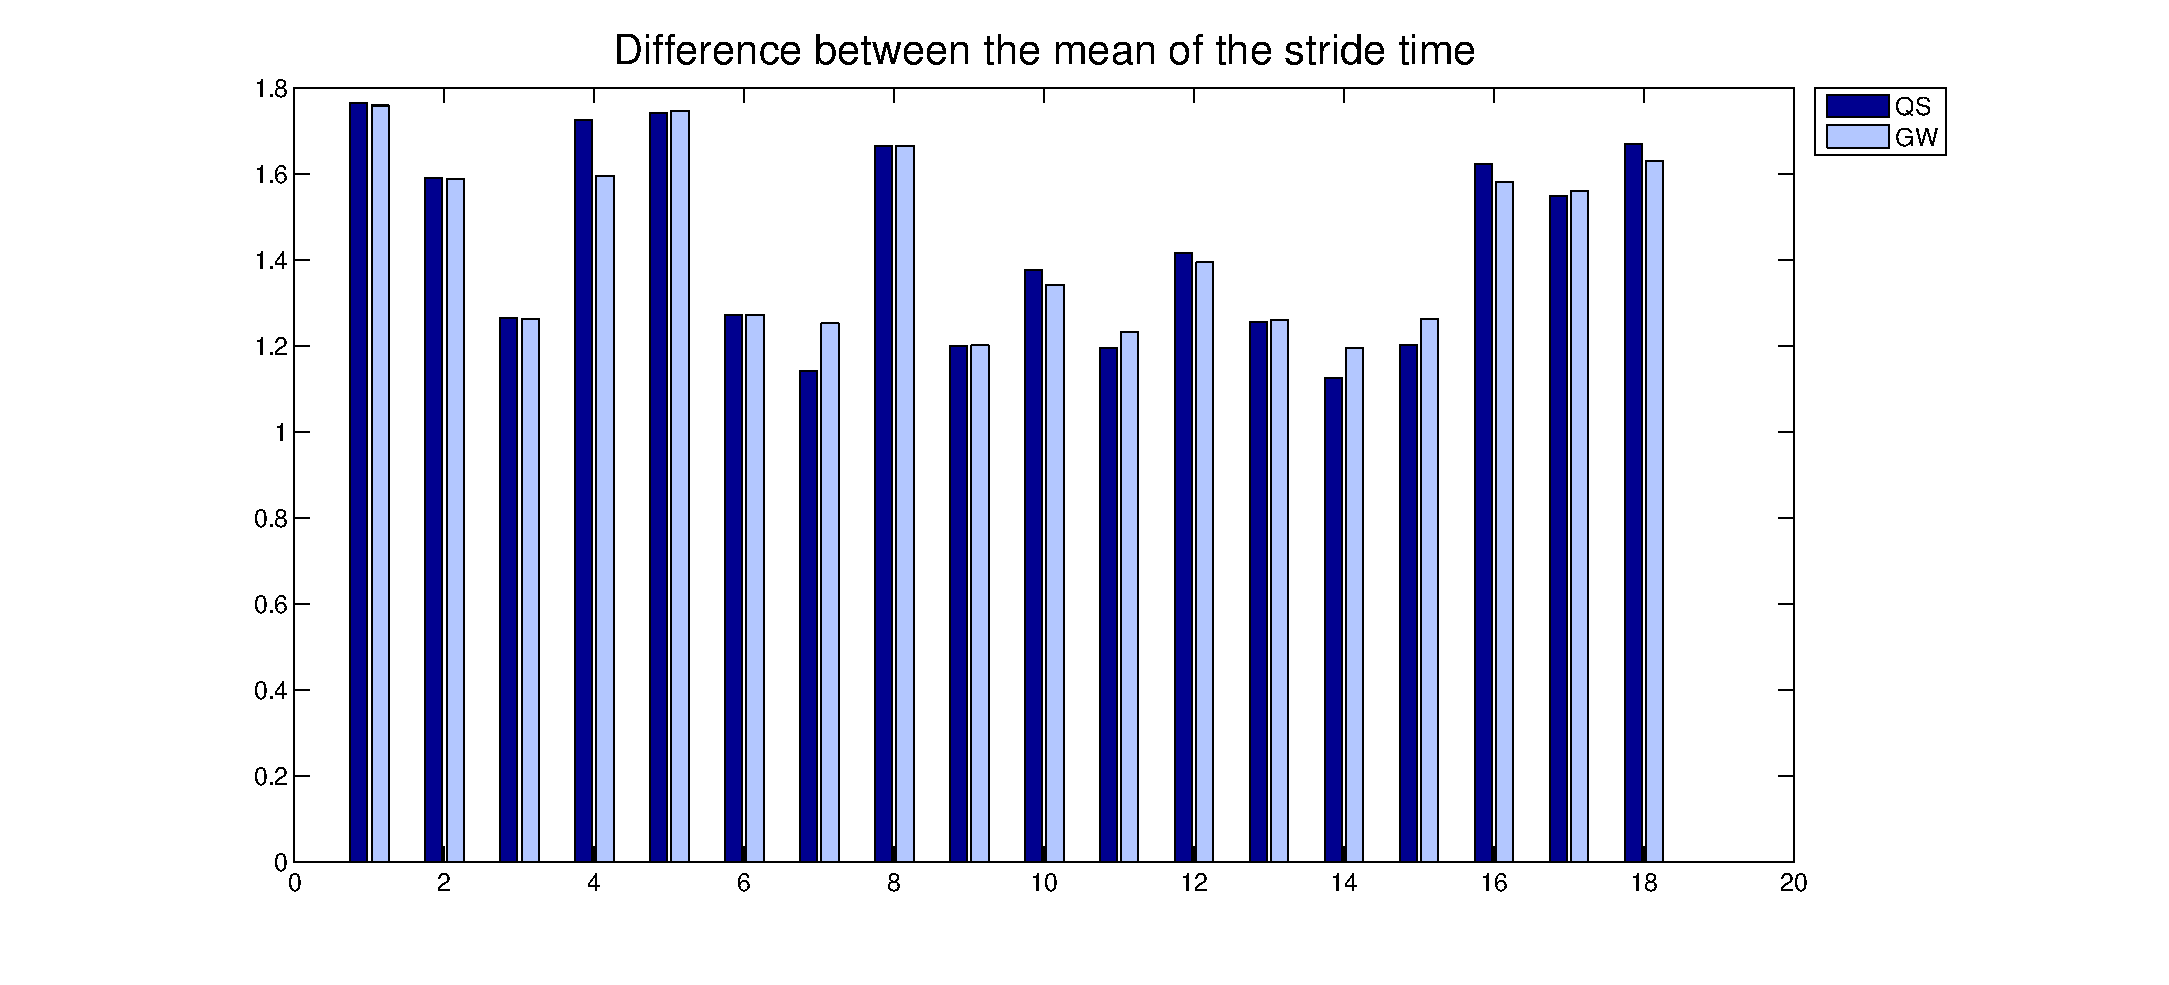
\epsfig{file=figures/QSvsGW/mean_stride_time, width=1\textwidth}
	\caption{Mean of the stride time for GW and QS signals.}
	\label{fig:mean_stride_time}
\end{figure}

‘Stride time’ is a feature used in a lot of experiments to characterise the movement because it is a interesting aspect that represents the time that a specific person needs to step. Also, it can be used for a classification between patients and control subjects, like in others studies \cite{Hausdorff}.
In our case, the difference between  the ‘stride time’ between both systems is very tiny. If we observe \ref{tab:Stride_time}, we can see that the greatest value of difference between systems is 0.1287 seconds.

\begin{table}[h]
	\caption{Comparation of the stride time and angle difference between GW and QS}	
	\centering
	\begin{tabular}{|c|c|c|}\hline
		
		Accomplishments & Difference Stride Time	& Difference Angle	 	\\ \hline
		1  & 0,006402343	 & 1,62502323 \\
		2 & 0,00214919	& 2,119358046 \\
		3 & 0,002432735	& 3,166649918 \\
		4 & 0,128717949	& 1,983148998 \\
		5 & 0,004818214	& 2,418373859 \\
		6 & 0,000302102	& 2,884211822 \\
		7 & 0,109688664	& 2,000748905 \\
		8 & 0,000282755	& 2,606004581 \\
		9 & 0,000604613	 & 0,644265922 \\
		10 & 0,034118318	& 2,093221696 \\
		11 & 0,038589012	& 2,597329501 \\
		12 & 0,022069119	& 0,039397798 \\
		13 & 0,004924869	& 2,771227548 \\
		14 & 0,069355008	& 2,87790541 \\
		15 & 0,059470686	& 2,227618016 \\
		16 & 0,041612352	& 0,511020994 \\
		17 & 0,012348426	& 1,834745133 \\
		18 & 0,039846301	& 1,701994772 
	\\ \hline
	\end{tabular}
	\label{tab:Stride_time}
	
\end{table}

\begin{table}[h]
	\caption{Features for different speeds}	
	\centering
	\begin{tabular}{|c|c|c|c|}\hline
		
		Speed & Stride time Diff Average & Stride time var Average & Angle Diff Average	 	\\ \hline
		2  & 1,6894	 & 0,00086 & 2,36 \\
		4 & 1,2397	& 0,017 & 4,1521\\
		6 & 1,4479 & 0,0094	& 4,6219
		\\ \hline
	\end{tabular}
	\label{tab:speeds}
	
\end{table}

In addition, it has been obtained the variations between the mean of the variance of the ‘stride time’. This parameter gives us information about the accuracy of both systems to calculate the pitch angle during the experiment.

In the majority of the accomplishments of the experiments, the variance of the GW system is greater than QS \ref{fig:var_stride_time}. It is probably due to the noise of the inertial sensors and the accuracy to calculate the pitch. However, they are very low values so it is not a important aspect that determine the quality against each other. 

\begin{figure}[H]
	\centering
	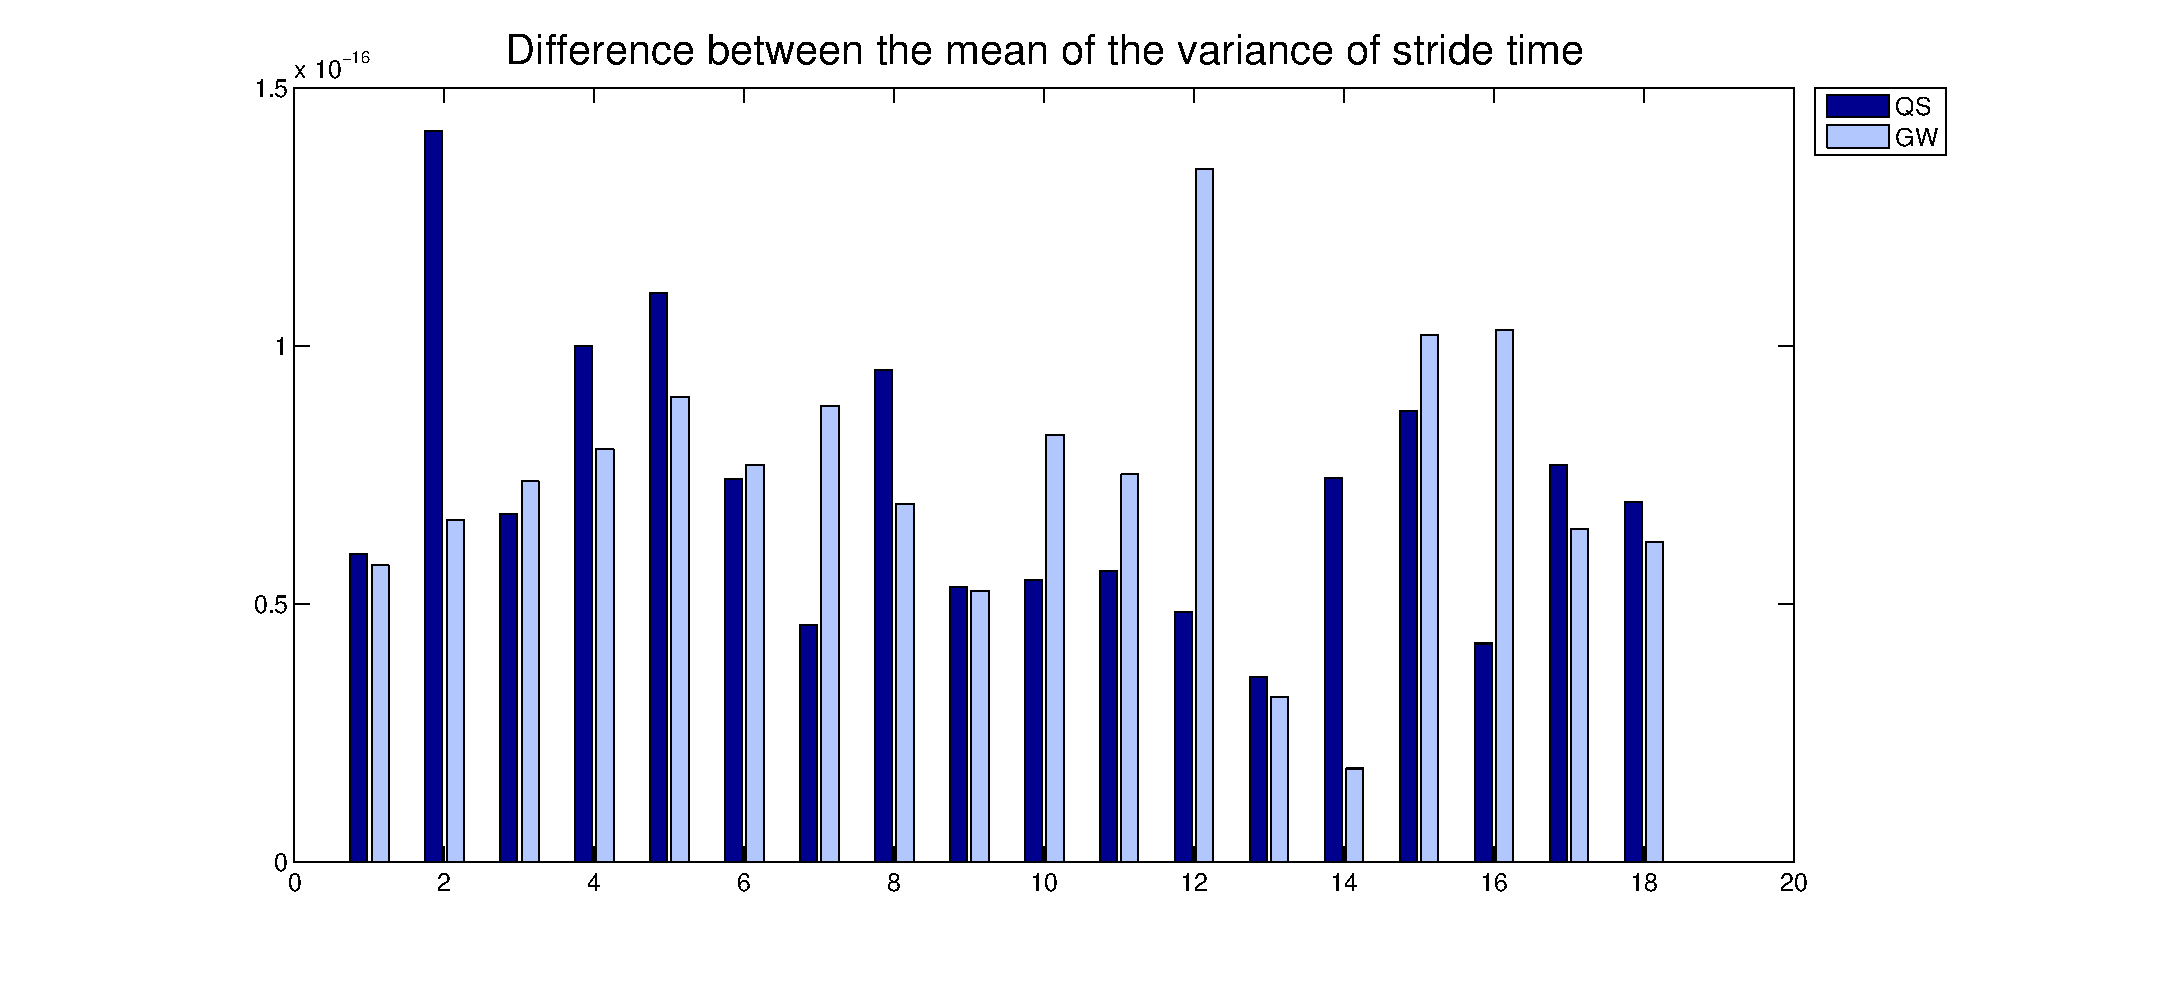
\epsfig{file=figures/QSvsGW/var_stride_time, width=1\textwidth}
	\caption{Mean of the stride time variance for GW and QS signals.}
	\label{fig:var_stride_time}
\end{figure}

Now, we will compare the mean of the angle in each experiment. The result of this is possible to see in \ref{fig:mean_angle}. It is clear that the differences aren’t too high. The greatest value of difference between angles is 3.16 degrees\ref{tab:Stride_time}. If we calculate the percentage with respect to the total average, this is about 12\% of the angle. This precision might be important depending on the application. In general, it doesn’t a significant value to characterise the movement. Therefore, Gait Watch system may be used to substitute the Qualisys systems as a good alternative regarding the accuracy, price and portability.

\begin{figure}[H]
	\centering
	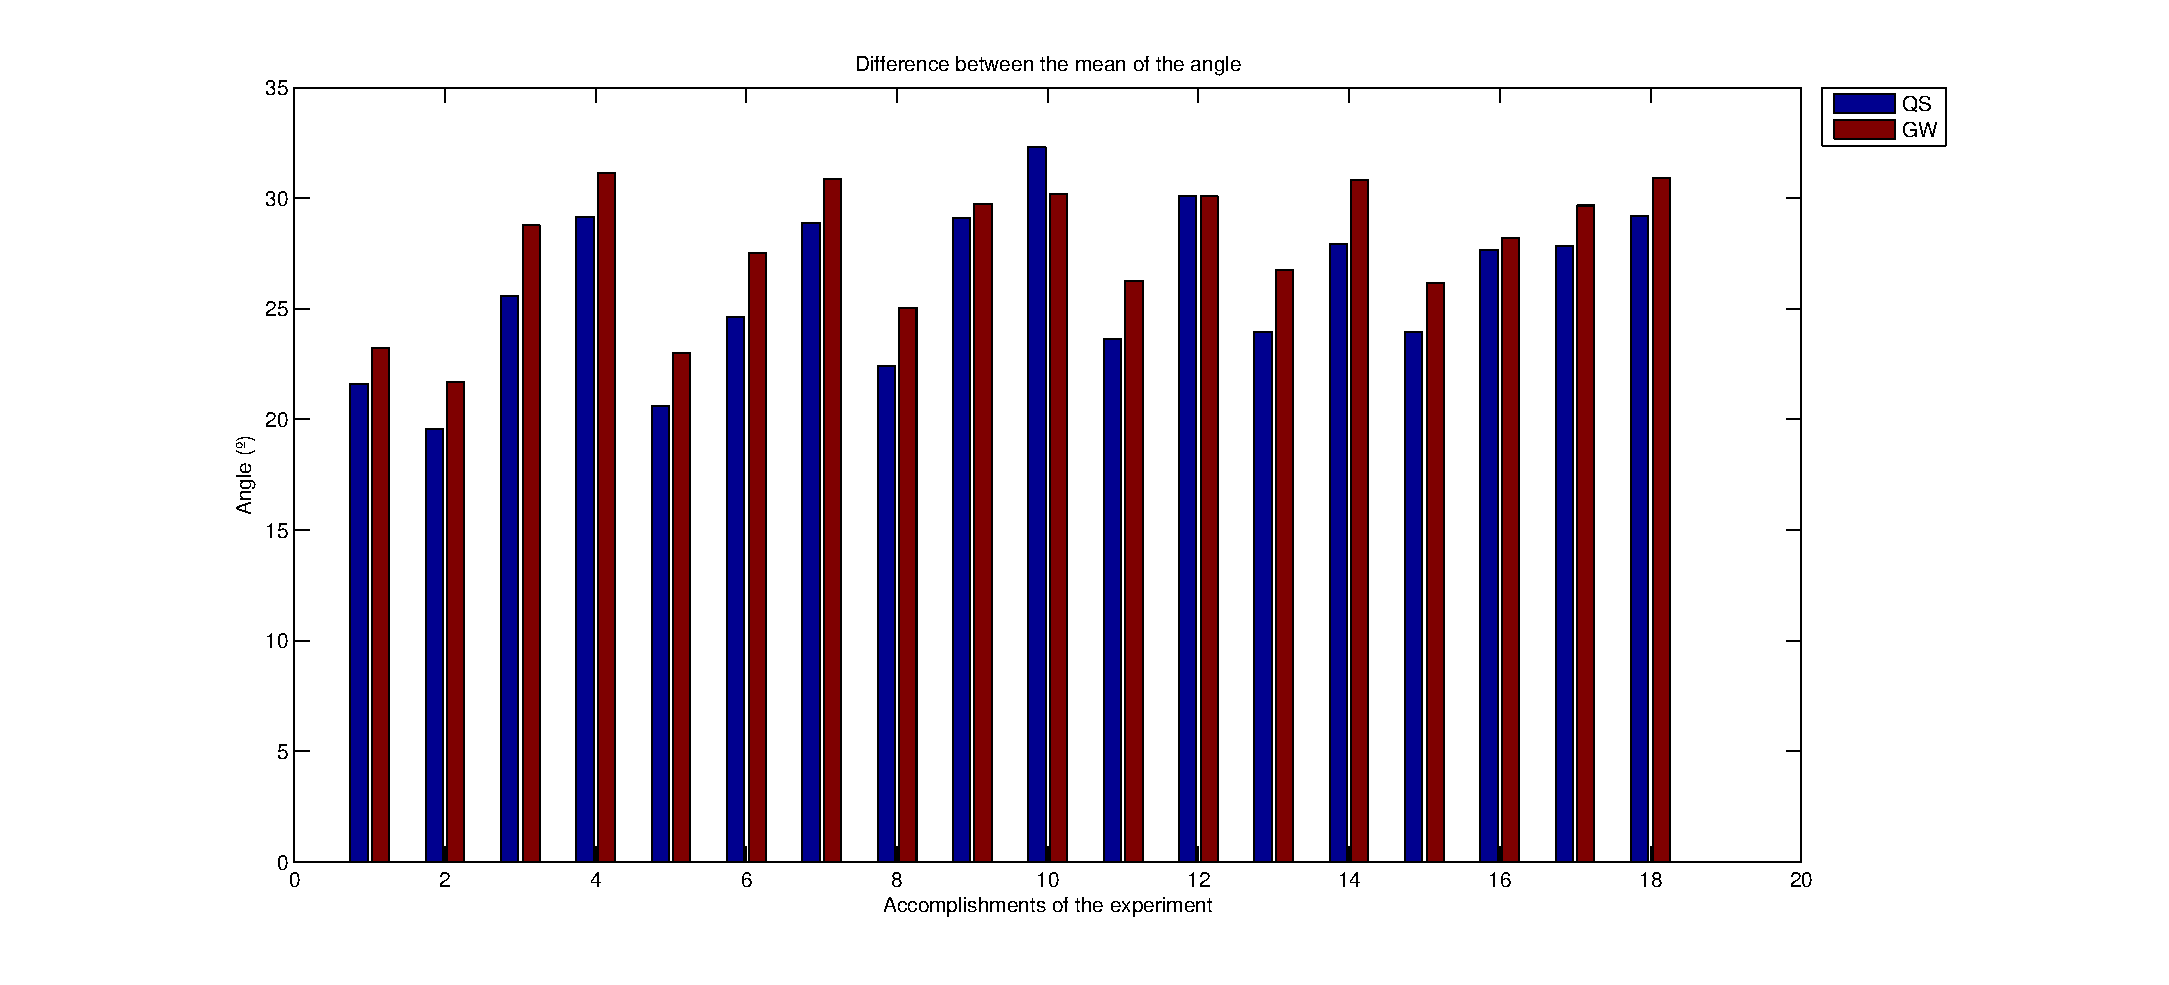
\epsfig{file=figures/QSvsGW/mean_angle, width=1\textwidth}
	\caption{Mean of the angle for GW and QS signals.}
	\label{fig:mean_angle}
\end{figure}

Then, we will see what happens when we analise the signals with regard to differents speeds. In \ref{fig:speed_stride_time}, we can see the mean of stride time for speeds of 2, 4 and 6 Km/h. If we have a look at the points represented in the picture, it seems that the ‘stride time’ is greater for low speeds than high speeds although it depends on the subject. In \ref{tab:speeds} it is shown the mean of all values for each velocity. The average ‘stride time’ is higer for 6Km/h than 4Km/h. However it does not happen in general. Therefore, we would need more measurements to stablish a final conclusion.

\begin{figure}[H]
	\centering
	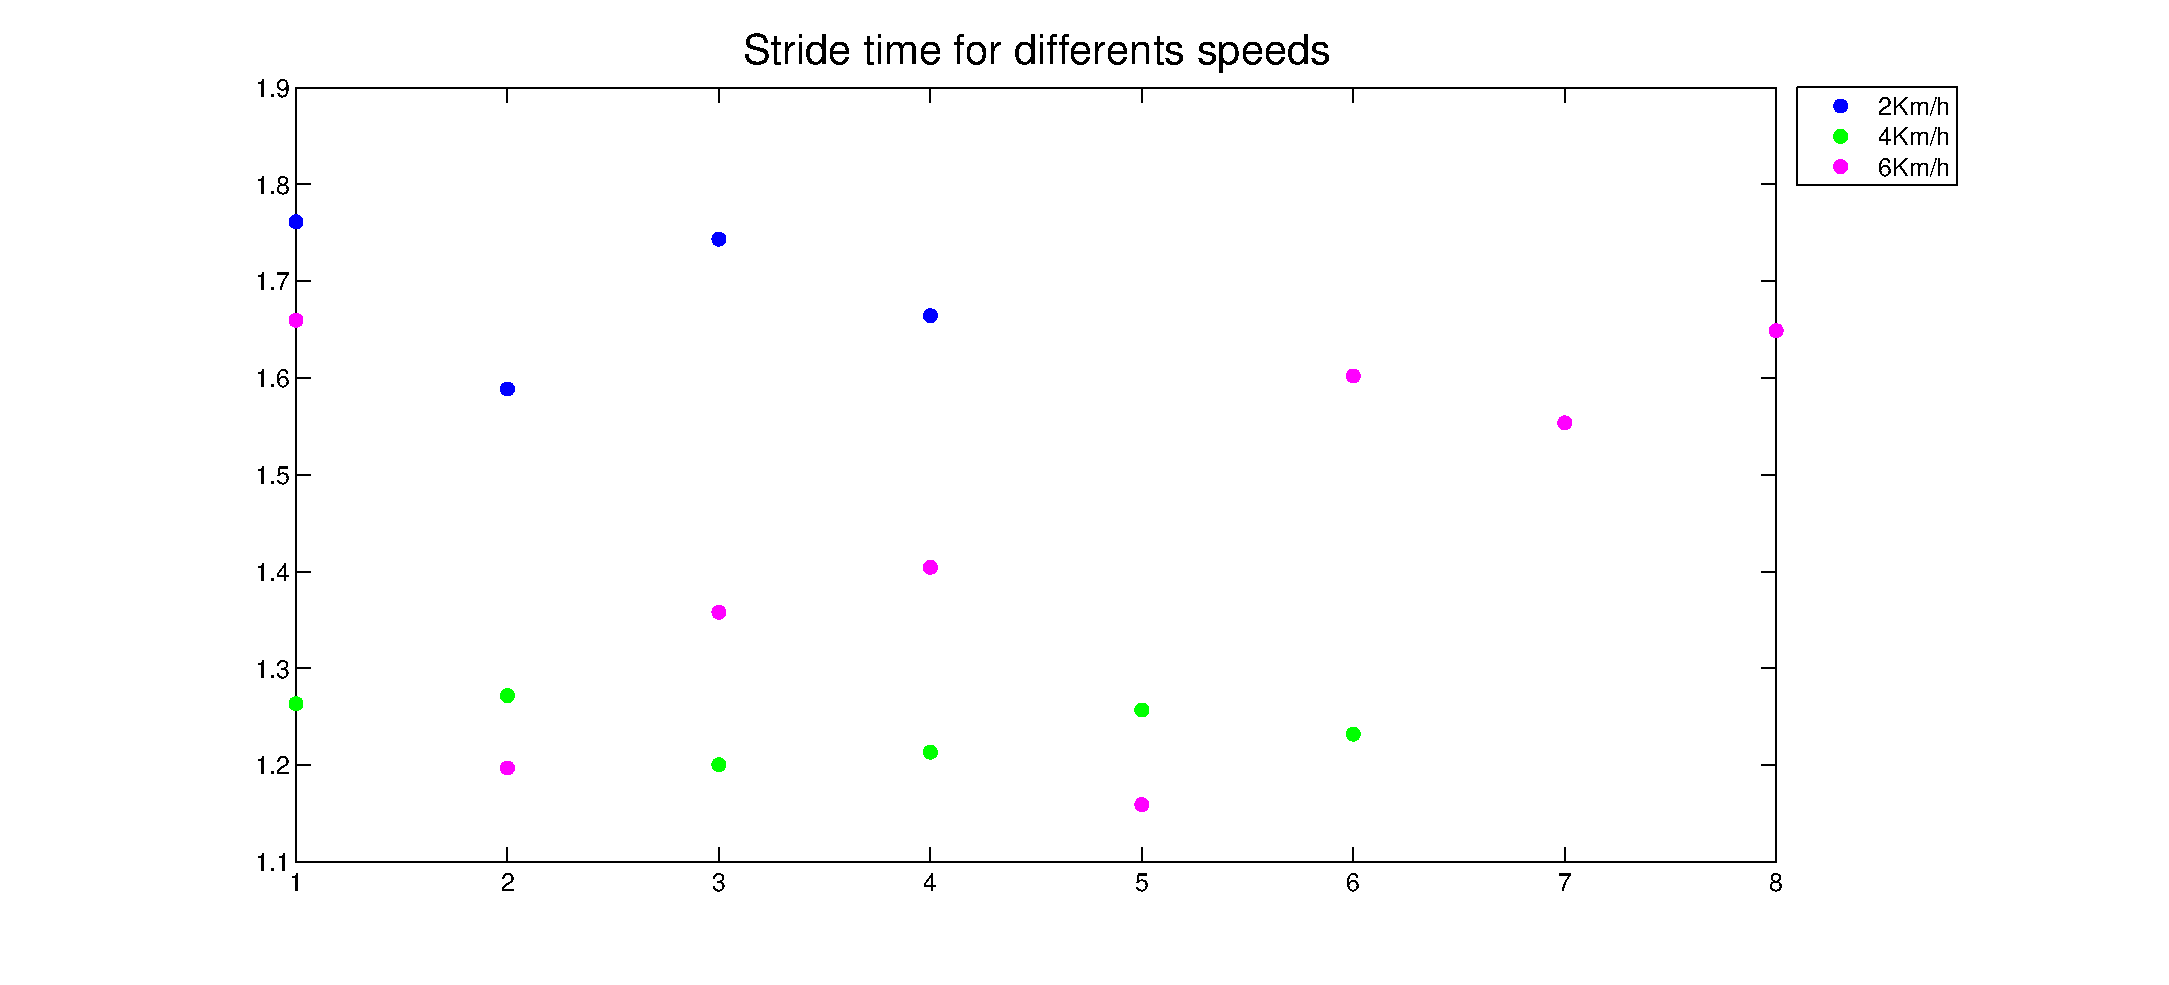
\epsfig{file=figures/QSvsGW/speed_stride_time, width=1\textwidth}
	\caption{Mean of stride time difference for each speeds.}
	\label{fig:speed_stride_time}
\end{figure}

\begin{figure}[H]
	\centering
	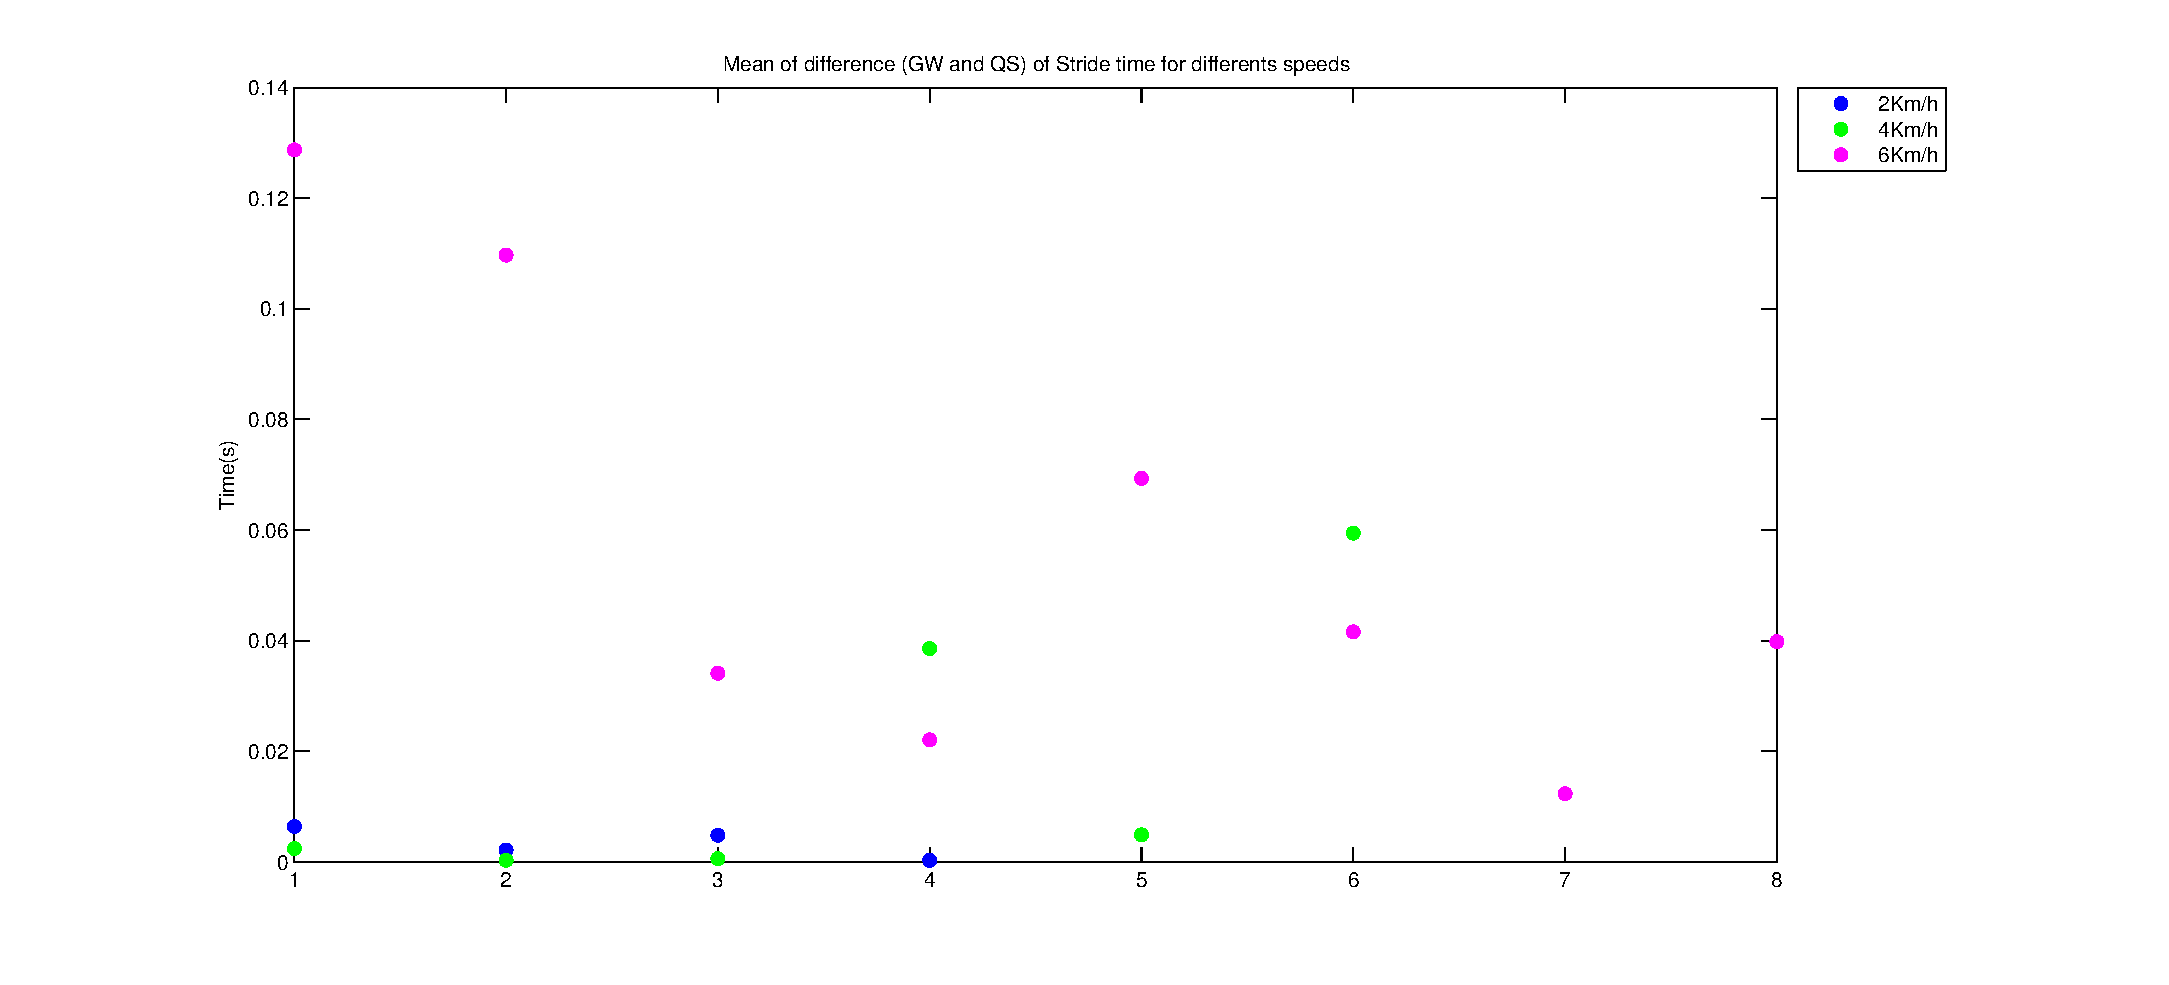
\epsfig{file=figures/QSvsGW/speed_var_stride_time, width=1\textwidth}
	\caption{Mean of stride time variance for each speeds.}
	\label{fig:speed_var_stride_time}
\end{figure}

If we scan \ref{fig:speed_var_stride_time}, we can appreciate the differences between the variance of ‘stride time’. Also, the mean of the values for each speed are put in the table \ref{tab:speeds} and the variance increases as the speed does it as well.

It is the same with the difference of the angle between systems \ref{fig:speed_angle}. The difference between angles increases with speed. So, it is an aspect that we have to consider for using the GW in place of QS.

\begin{figure}[H]
	\centering
	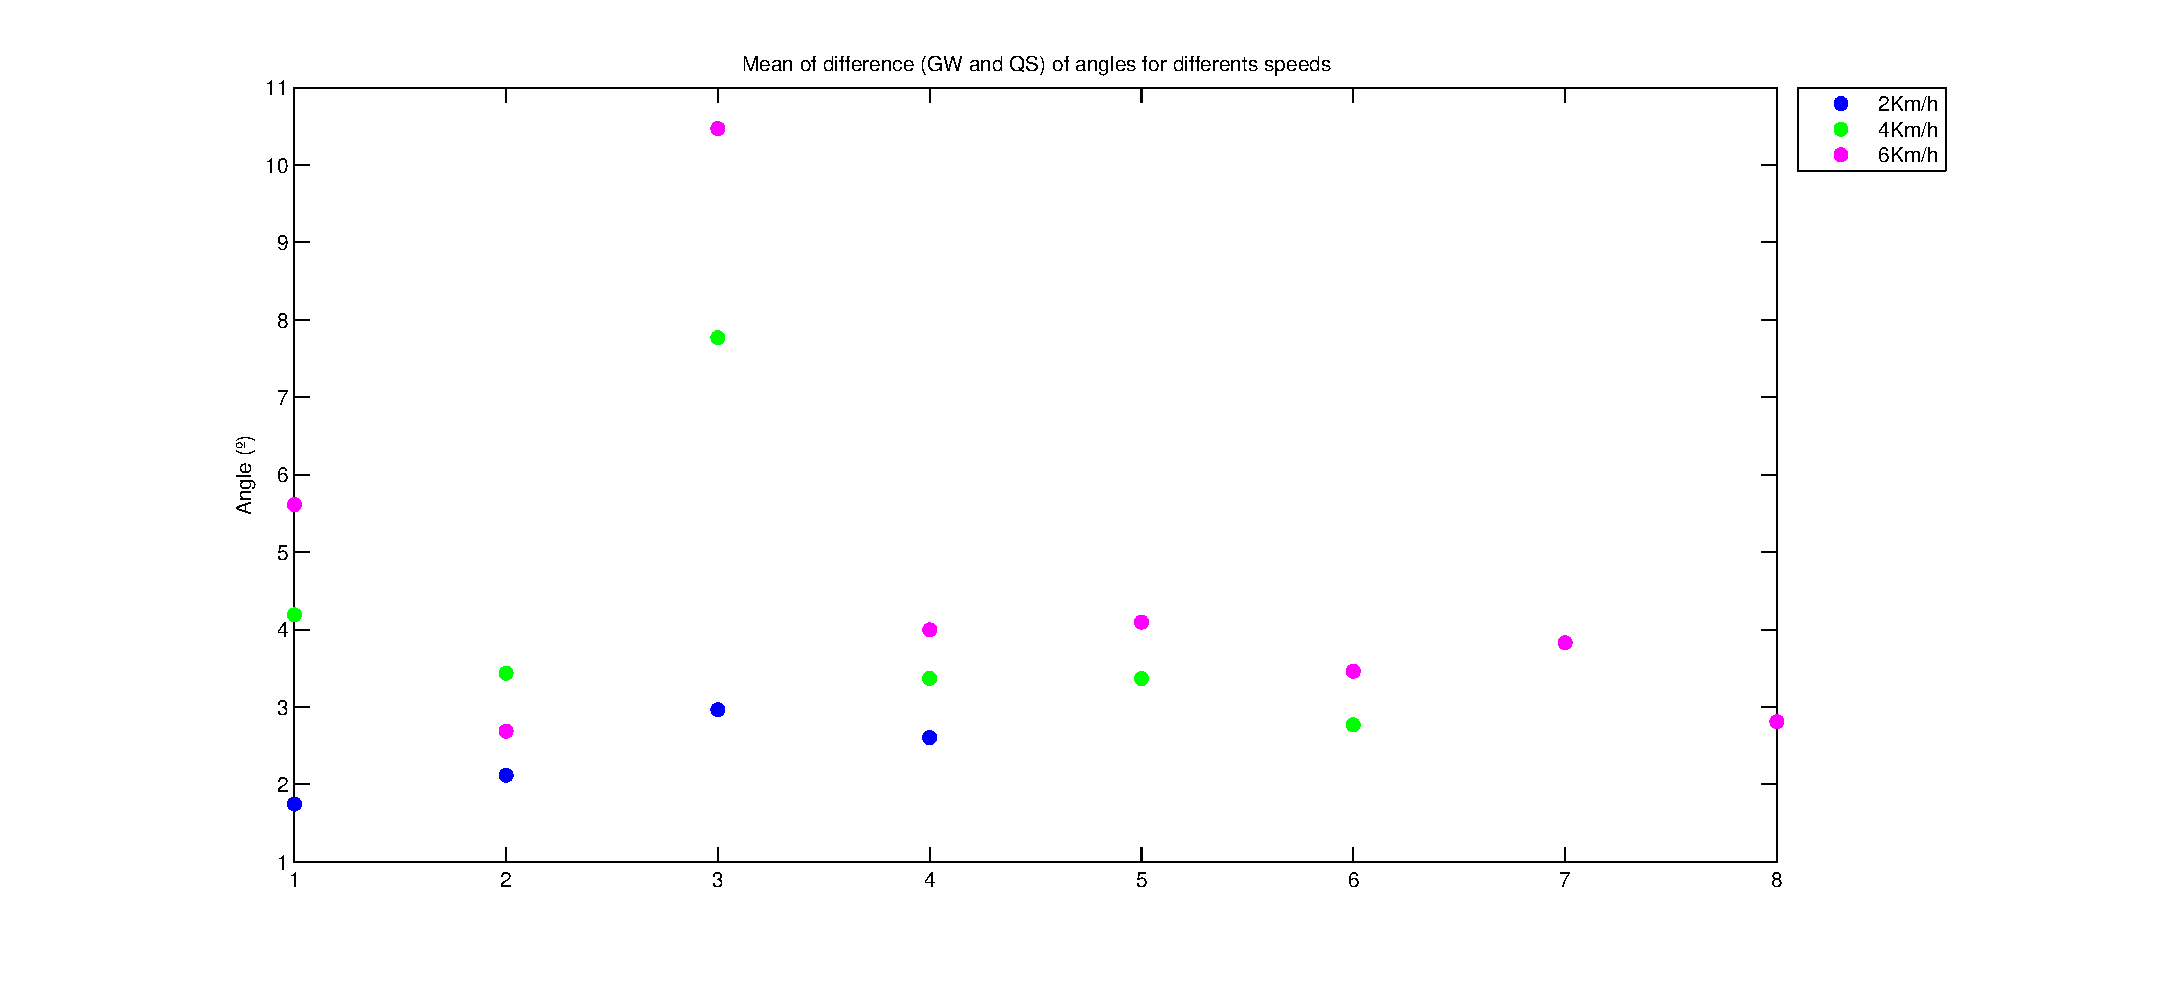
\epsfig{file=figures/QSvsGW/speed_angle, width=1\textwidth}
	\caption{Mean of angle difference for each speeds.}
	\label{fig:speed_angle}
\end{figure}


